\documentclass[UTF8,zihao=-4]{ctexart}
\usepackage[a4paper,margin=2.5cm]{geometry}
\usepackage{amsmath, amssymb, amsthm}
\usepackage{bm}
\usepackage{hyperref}
\usepackage{graphicx}
\usepackage{caption}
\usepackage{listings}
\usepackage{xcolor}
\usepackage{float}
\usepackage{placeins}
\graphicspath{{figures/}}

% Code style
\lstdefinestyle{code}{
  basicstyle=\ttfamily\small,
  numbers=left,
  numberstyle=\tiny,
  numbersep=8pt,
  keywordstyle=\color{blue},
  commentstyle=\color{teal!70!black},
  stringstyle=\color{orange!70!black},
  showstringspaces=false,
  breaklines=true,
  frame=single,
  framerule=0.3pt,
  rulecolor=\color{black!15}
}
\lstset{style=code}

\title{图神经网络:GCN 基础与典型应用}
\author{}
\date{\today}

\begin{document}
\maketitle
\tableofcontents
\FloatBarrier

\section{图卷积网络(GCN)}
图卷积网络将卷积思想推广到非欧氏结构的图数据。在无向图 $G = (\mathcal{V}, \mathcal{E})$ 中,设邻接矩阵为 $\mathbf{A}$,节点特征矩阵为 $\mathbf{X} \in \mathbb{R}^{|\mathcal{V}| \times d}$。谱图理论为卷积定义提供了形式化框架。图~\ref{fig:gcn_graph_structure_cn} 概述了邻居聚合的流程。

\subsection{谱域定义}
组合拉普拉斯矩阵 $\mathbf{L} = \mathbf{D} - \mathbf{A}$($\mathbf{D}$ 为度矩阵)可分解为 $\mathbf{L} = \mathbf{U} \boldsymbol{\Lambda} \mathbf{U}^\top$。谱滤波 $g_\theta(\boldsymbol{\Lambda})$ 作用于信号 $\mathbf{X}$ 的结果为
\begin{equation}
  g_\theta \star \mathbf{X} = \mathbf{U} g_\theta(\boldsymbol{\Lambda}) \mathbf{U}^\top \mathbf{X}.
\end{equation}
利用切比雪夫多项式近似 $g_\theta$,得到 $K$ 跳邻域支持:
\begin{equation}
  g_\theta \star \mathbf{X} \approx \sum_{k=0}^{K} \theta_k T_k(\tilde{\mathbf{L}})\mathbf{X}, \quad \tilde{\mathbf{L}} = \frac{2}{\lambda_{\max}} \mathbf{L} - \mathbf{I}.
\end{equation}
Kipf \& Welling 将其简化为一阶形式($K=1$),并通过自环重归一化:
\begin{equation}
  \mathbf{H}^{(l+1)} = \sigma\left(\tilde{\mathbf{D}}^{-1/2} \tilde{\mathbf{A}} \tilde{\mathbf{D}}^{-1/2} \mathbf{H}^{(l)} \mathbf{W}^{(l)}\right),
\end{equation}
其中 $\tilde{\mathbf{A}} = \mathbf{A} + \mathbf{I}$,$\tilde{\mathbf{D}}_{ii} = \sum_j \tilde{\mathbf{A}}_{ij}$。对称归一化保证了数值稳定性,并包含自身节点信息。

\subsection{信息传递视角}
从消息传递角度看,GCN 层通过邻居特征平均更新节点:
\begin{equation}
  \mathbf{h}_v^{(l+1)} = \sigma\left(\sum_{u \in \mathcal{N}(v) \cup \{v\}} \frac{1}{\sqrt{\tilde{d}_v \tilde{d}_u}} \mathbf{h}_u^{(l)} \mathbf{W}^{(l)}\right),
\end{equation}
其中 $\tilde{d}_v$ 为加入自环后的度。图~\ref{fig:gcn_layer_flow_cn} 展示了两层 GCN 的信息传播范围。

\subsection{过平滑与缓解}
随着层数增加,节点表示趋于一致,即“过平滑”。常见缓解方法:
\begin{itemize}
  \item 引入残差/跳连(Res-GCN、JK-Net)保留低阶特征。
  \item 使用正则化归一(PairNorm、BatchNorm)稳定嵌入方差。
  \item 个性化传播(APPNP)结合随机游走与抛掷概率:
  \begin{equation}
    \mathbf{Z} = (1-\alpha) (\mathbf{I} - \alpha \tilde{\mathbf{P}})^{-1} \mathbf{H}^{(K)}, \quad \tilde{\mathbf{P}} = \tilde{\mathbf{D}}^{-1} \tilde{\mathbf{A}}.
  \end{equation}
\end{itemize}

\subsection{训练流程}
\begin{lstlisting}[language=Python, caption={基于 PyTorch Geometric 的半监督二维 GCN 节点分类示例。}]
import torch
import torch.nn.functional as F
from torch_geometric.nn import GCNConv

class GCN(torch.nn.Module):
    def __init__(self, in_dim, hidden_dim, out_dim, dropout=0.5):
        super().__init__()
        self.conv1 = GCNConv(in_dim, hidden_dim, normalize=True)
        self.conv2 = GCNConv(hidden_dim, out_dim, normalize=True)
        self.dropout = dropout

    def forward(self, x, edge_index):
        x = self.conv1(x, edge_index)
        x = F.relu(x)
        x = F.dropout(x, p=self.dropout, training=self.training)
        x = self.conv2(x, edge_index)
        return F.log_softmax(x, dim=1)

model = GCN(dataset.num_node_features, 64, dataset.num_classes)
optimizer = torch.optim.Adam(model.parameters(), lr=0.01, weight_decay=5e-4)

for epoch in range(200):
    model.train()
    optimizer.zero_grad()
    out = model(data.x, data.edge_index)
    loss = F.nll_loss(out[data.train_mask], data.y[data.train_mask])
    loss.backward()
    optimizer.step()
\end{lstlisting}

\begin{figure}[H]
  \centering
  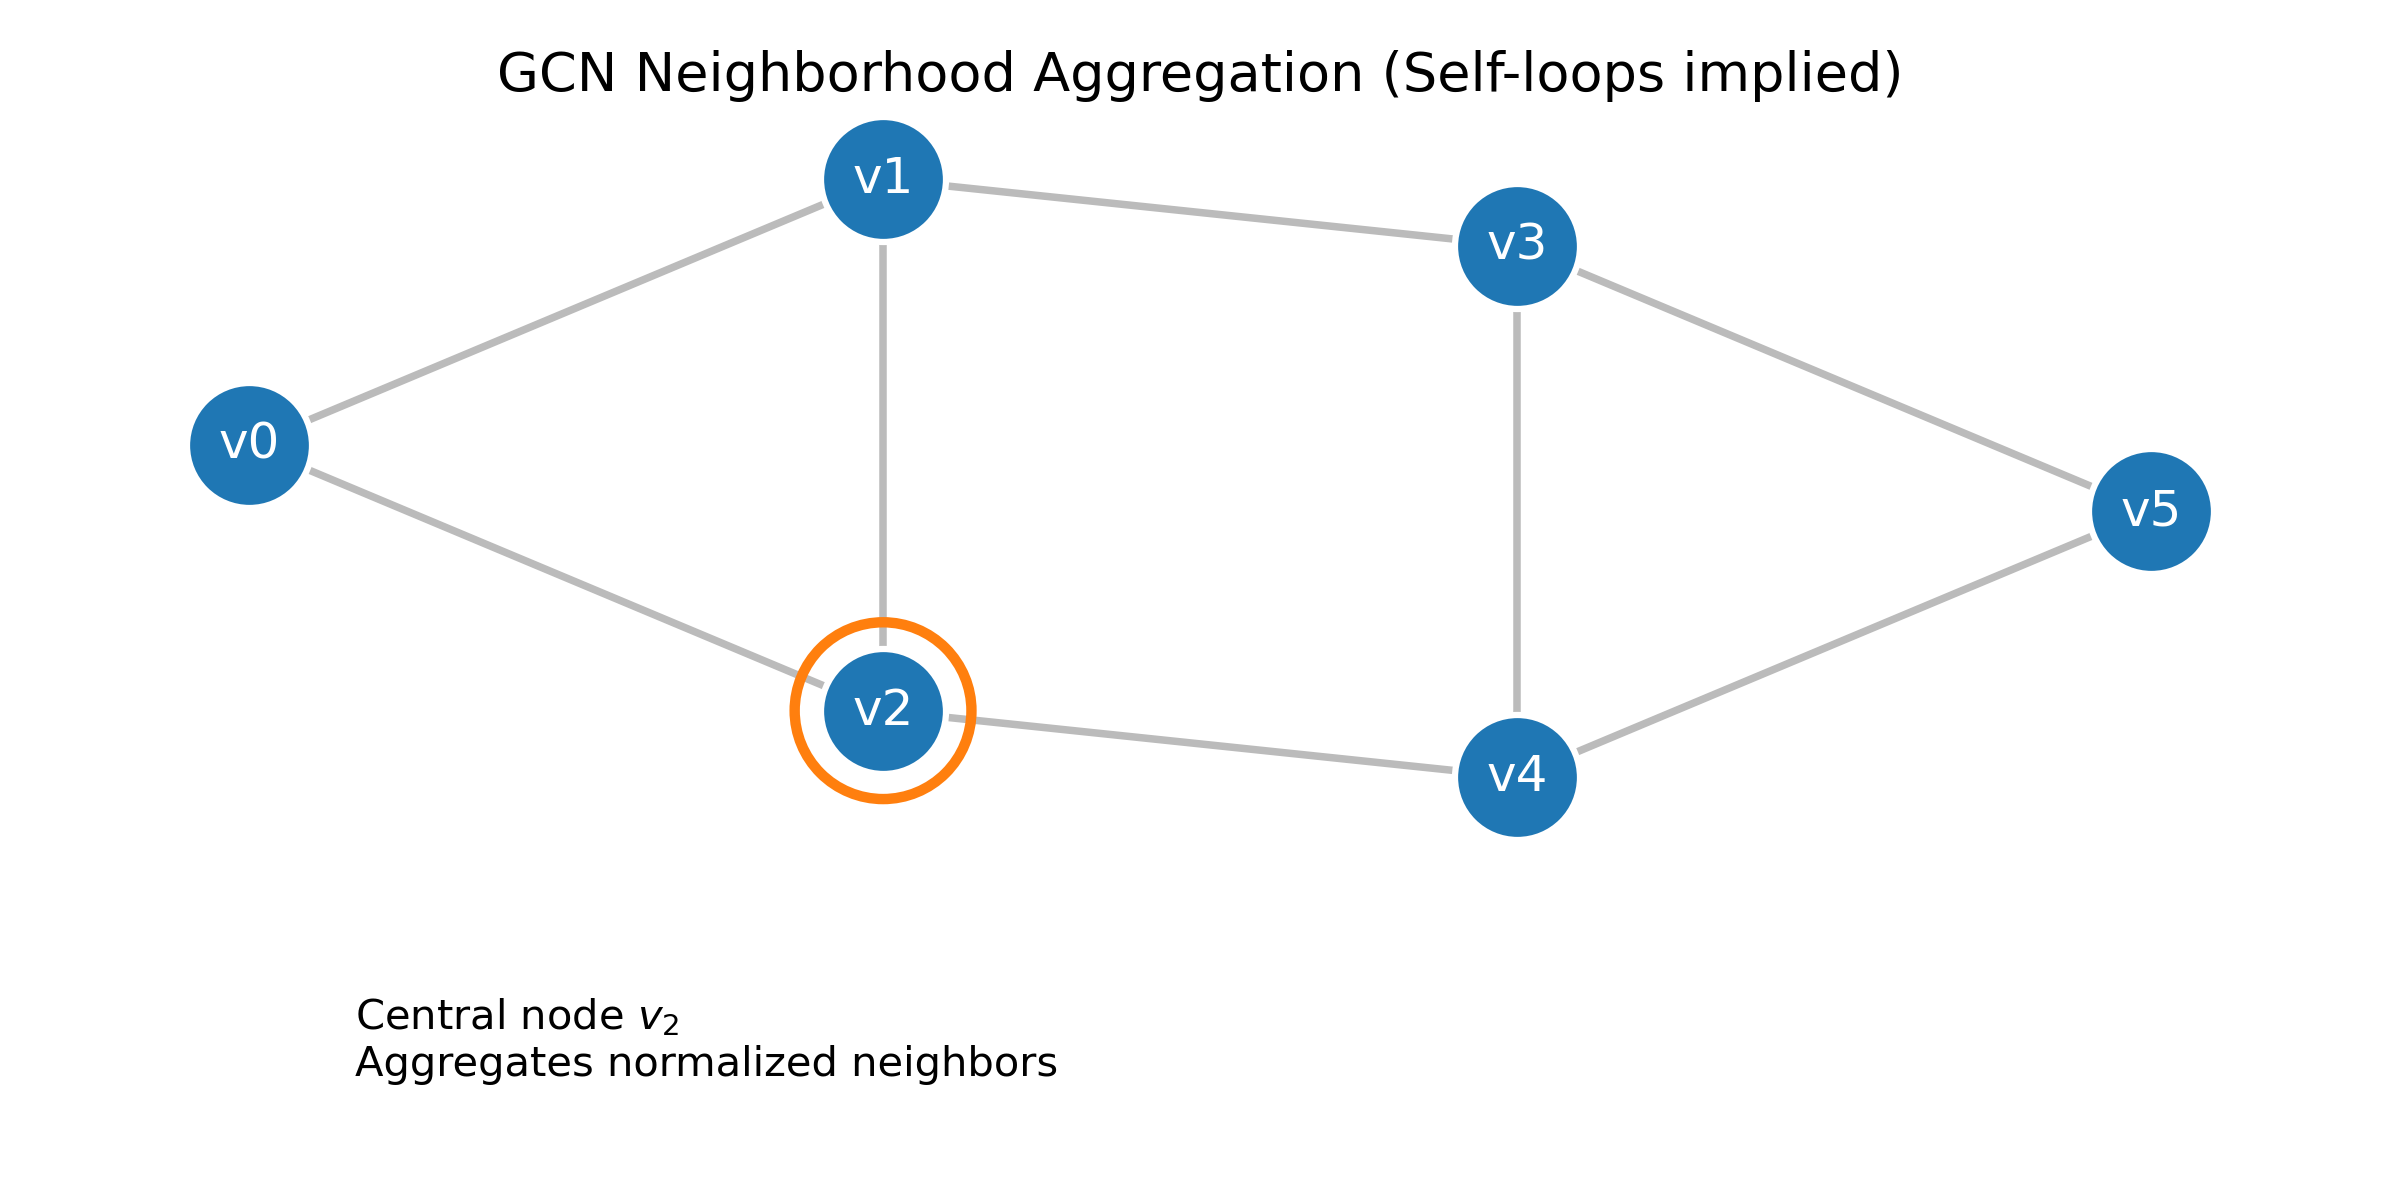
\includegraphics[width=0.75\textwidth]{gcn_graph_structure.png}
  \caption{图卷积使用归一化邻域聚合,包含自环信息以避免特征缺失。}
  \label{fig:gcn_graph_structure_cn}
\end{figure}

\begin{figure}[H]
  \centering
  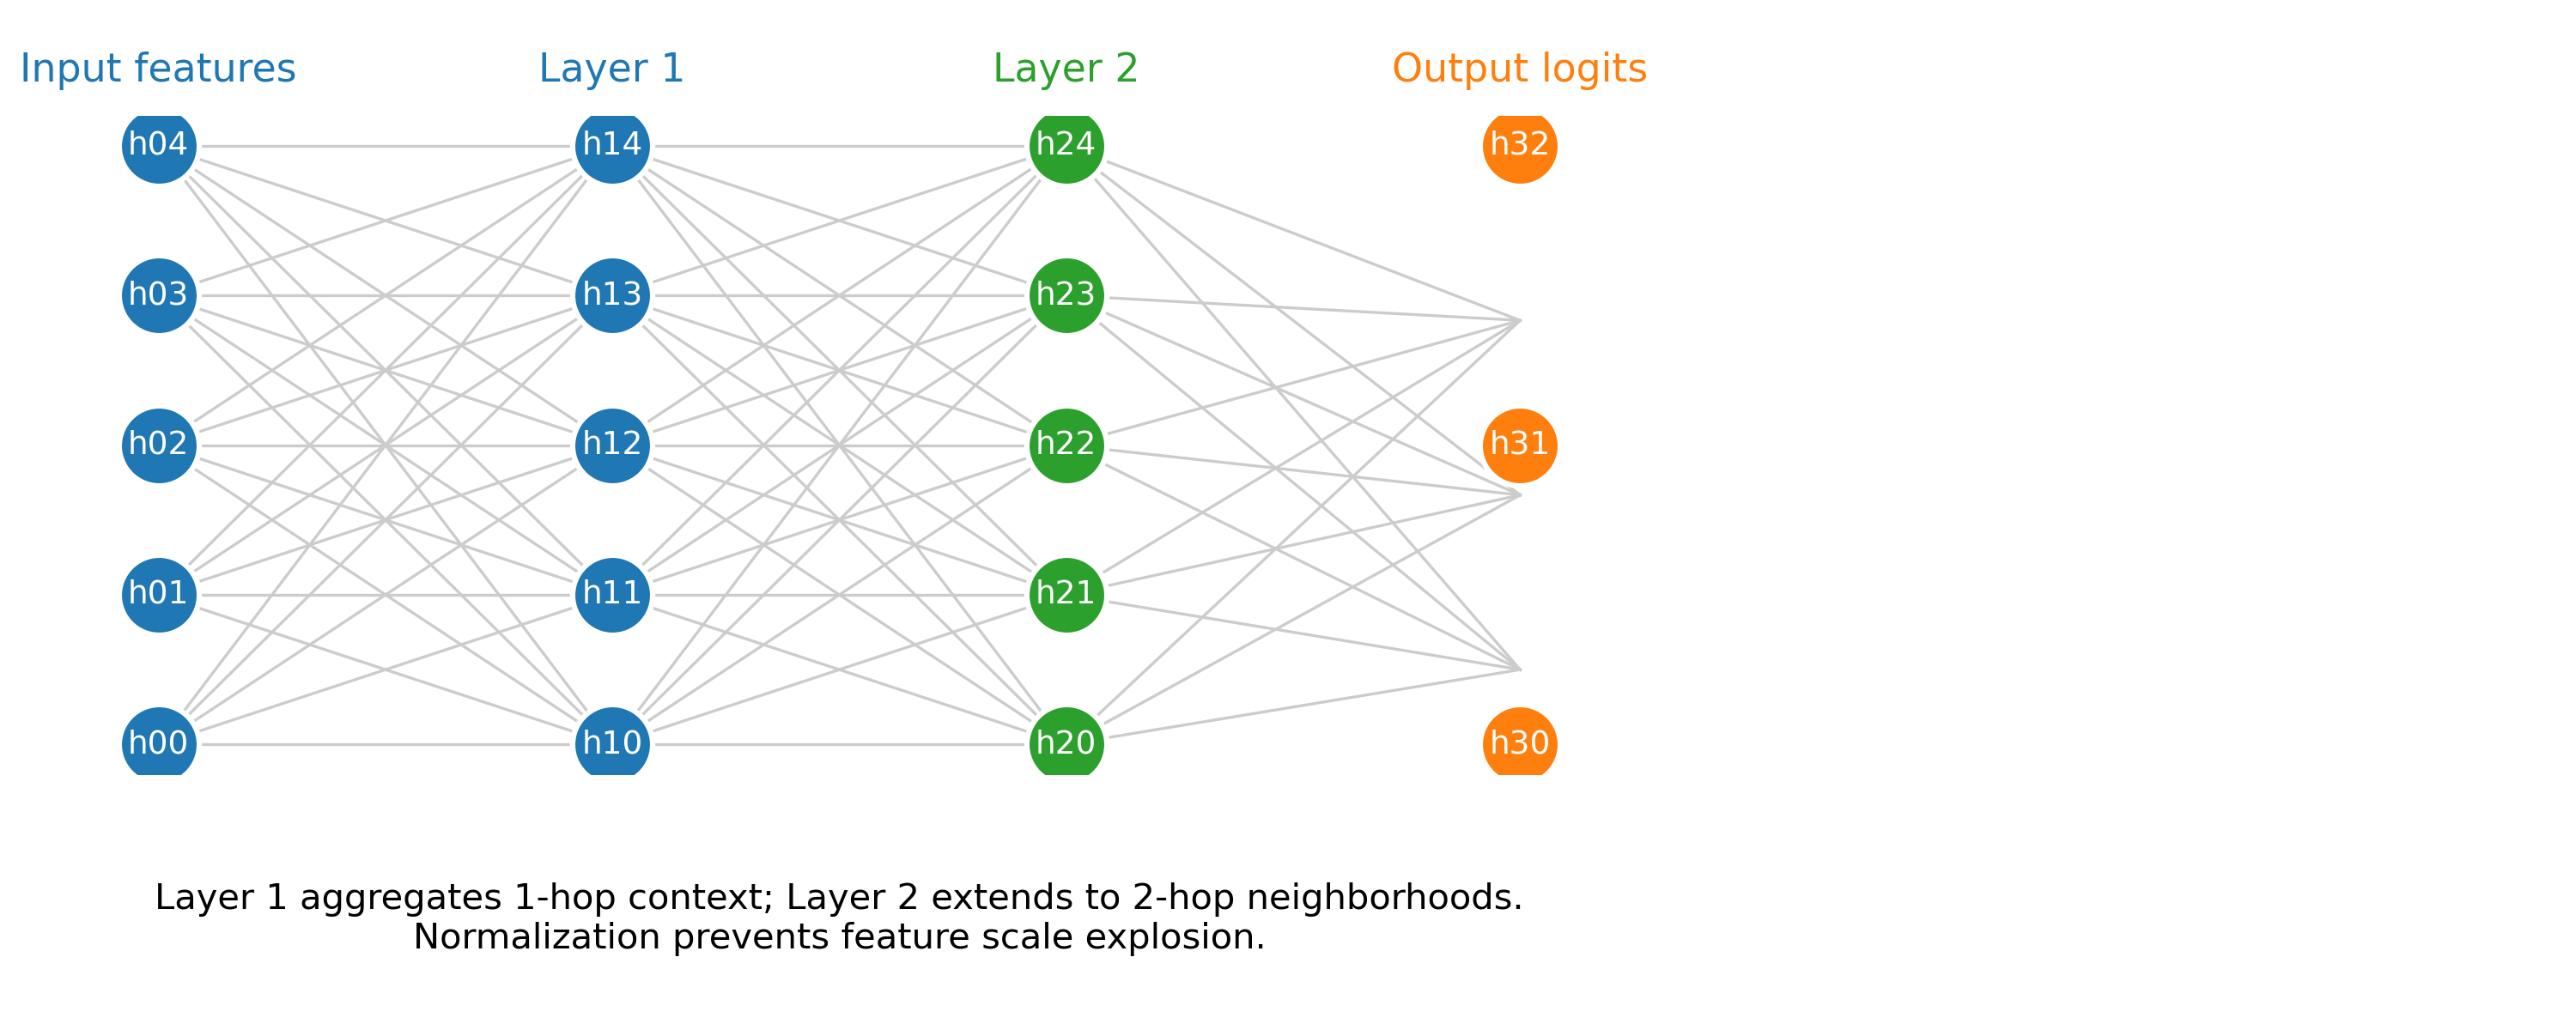
\includegraphics[width=0.85\textwidth]{gcn_layer_flow.png}
  \caption{两层 GCN 的信息范围示意:第一层覆盖一跳邻居,第二层扩展至两跳。}
  \label{fig:gcn_layer_flow_cn}
\end{figure}
\FloatBarrier

\section{应用:社交网络、分子预测、推荐系统}
GCN 及广义图神经网络在多种关系数据场景中表现突出。图~\ref{fig:gnn_application_landscape_cn} 描绘了典型应用流程。

\subsection{社交网络分析}
社交图中,GCN 能够结合相似性与结构信息学习用户嵌入,用于社区发现、影响力预测、内容推荐。对于包含多类型节点/边的异构图,可使用关系图卷积网络(R-GCN):
\begin{equation}
  \mathbf{h}_v^{(l+1)} = \sigma \left( \sum_{r \in \mathcal{R}} \sum_{u \in \mathcal{N}_r(v)} \frac{1}{c_{v,r}} \mathbf{W}_r^{(l)} \mathbf{h}_u^{(l)} + \mathbf{W}_0^{(l)} \mathbf{h}_v^{(l)} \right).
\end{equation}
在大规模平台上,需要 GraphSAGE、Cluster-GCN 等采样技术以控制算力开销。

\subsection{分子性质预测}
分子可视作节点为原子、边为化学键的图。消息传递神经网络(MPNN)在 GCN 基础上引入边特征:
\begin{align}
  \mathbf{m}_v^{(l+1)} &= \sum_{u \in \mathcal{N}(v)} \phi^{(l)}\left(\mathbf{h}_v^{(l)}, \mathbf{h}_u^{(l)}, \mathbf{e}_{uv}\right), \\
  \mathbf{h}_v^{(l+1)} &= \psi^{(l)}\left(\mathbf{h}_v^{(l)}, \mathbf{m}_v^{(l+1)}\right),
\end{align}
其中 $\mathbf{e}_{uv}$ 表示键类型/长度。全局池化(求和、平均、set2set)将节点嵌入汇总为分子指纹。结合等变网络(E(n)-GNN)与量子化特征,可在 QM9、Materials Project 等数据集取得领先结果。

\subsection{推荐系统}
用户-物品交互形成二部图。LightGCN 移除非线性与特征变换,简化传播:
\begin{equation}
  \mathbf{E}^{(k+1)} = \tilde{\mathbf{D}}^{-1/2} \tilde{\mathbf{A}} \tilde{\mathbf{D}}^{-1/2} \mathbf{E}^{(k)}, \qquad \mathbf{E} = \frac{1}{K+1} \sum_{k=0}^{K} \mathbf{E}^{(k)}.
\end{equation}
最终嵌入用于打分 $s_{ui} = \mathbf{e}_u^\top \mathbf{e}_i$。真实业务场景还需考虑时间因素、内容特征及因果去偏。

\subsection{部署与工程实践}
\begin{itemize}
  \item \textbf{可扩展性:} PinSAGE、GraphSAINT 利用随机游走采样;图划分、分布式训练支撑十亿级边。
  \item \textbf{可解释性:} GNNExplainer、GraphMask 等方法突出关键子图,提高模型透明度。
  \item \textbf{鲁棒性:} 针对对抗攻击的防御方法包括对抗训练、随机平滑认证等。
\end{itemize}

\begin{figure}[H]
  \centering
  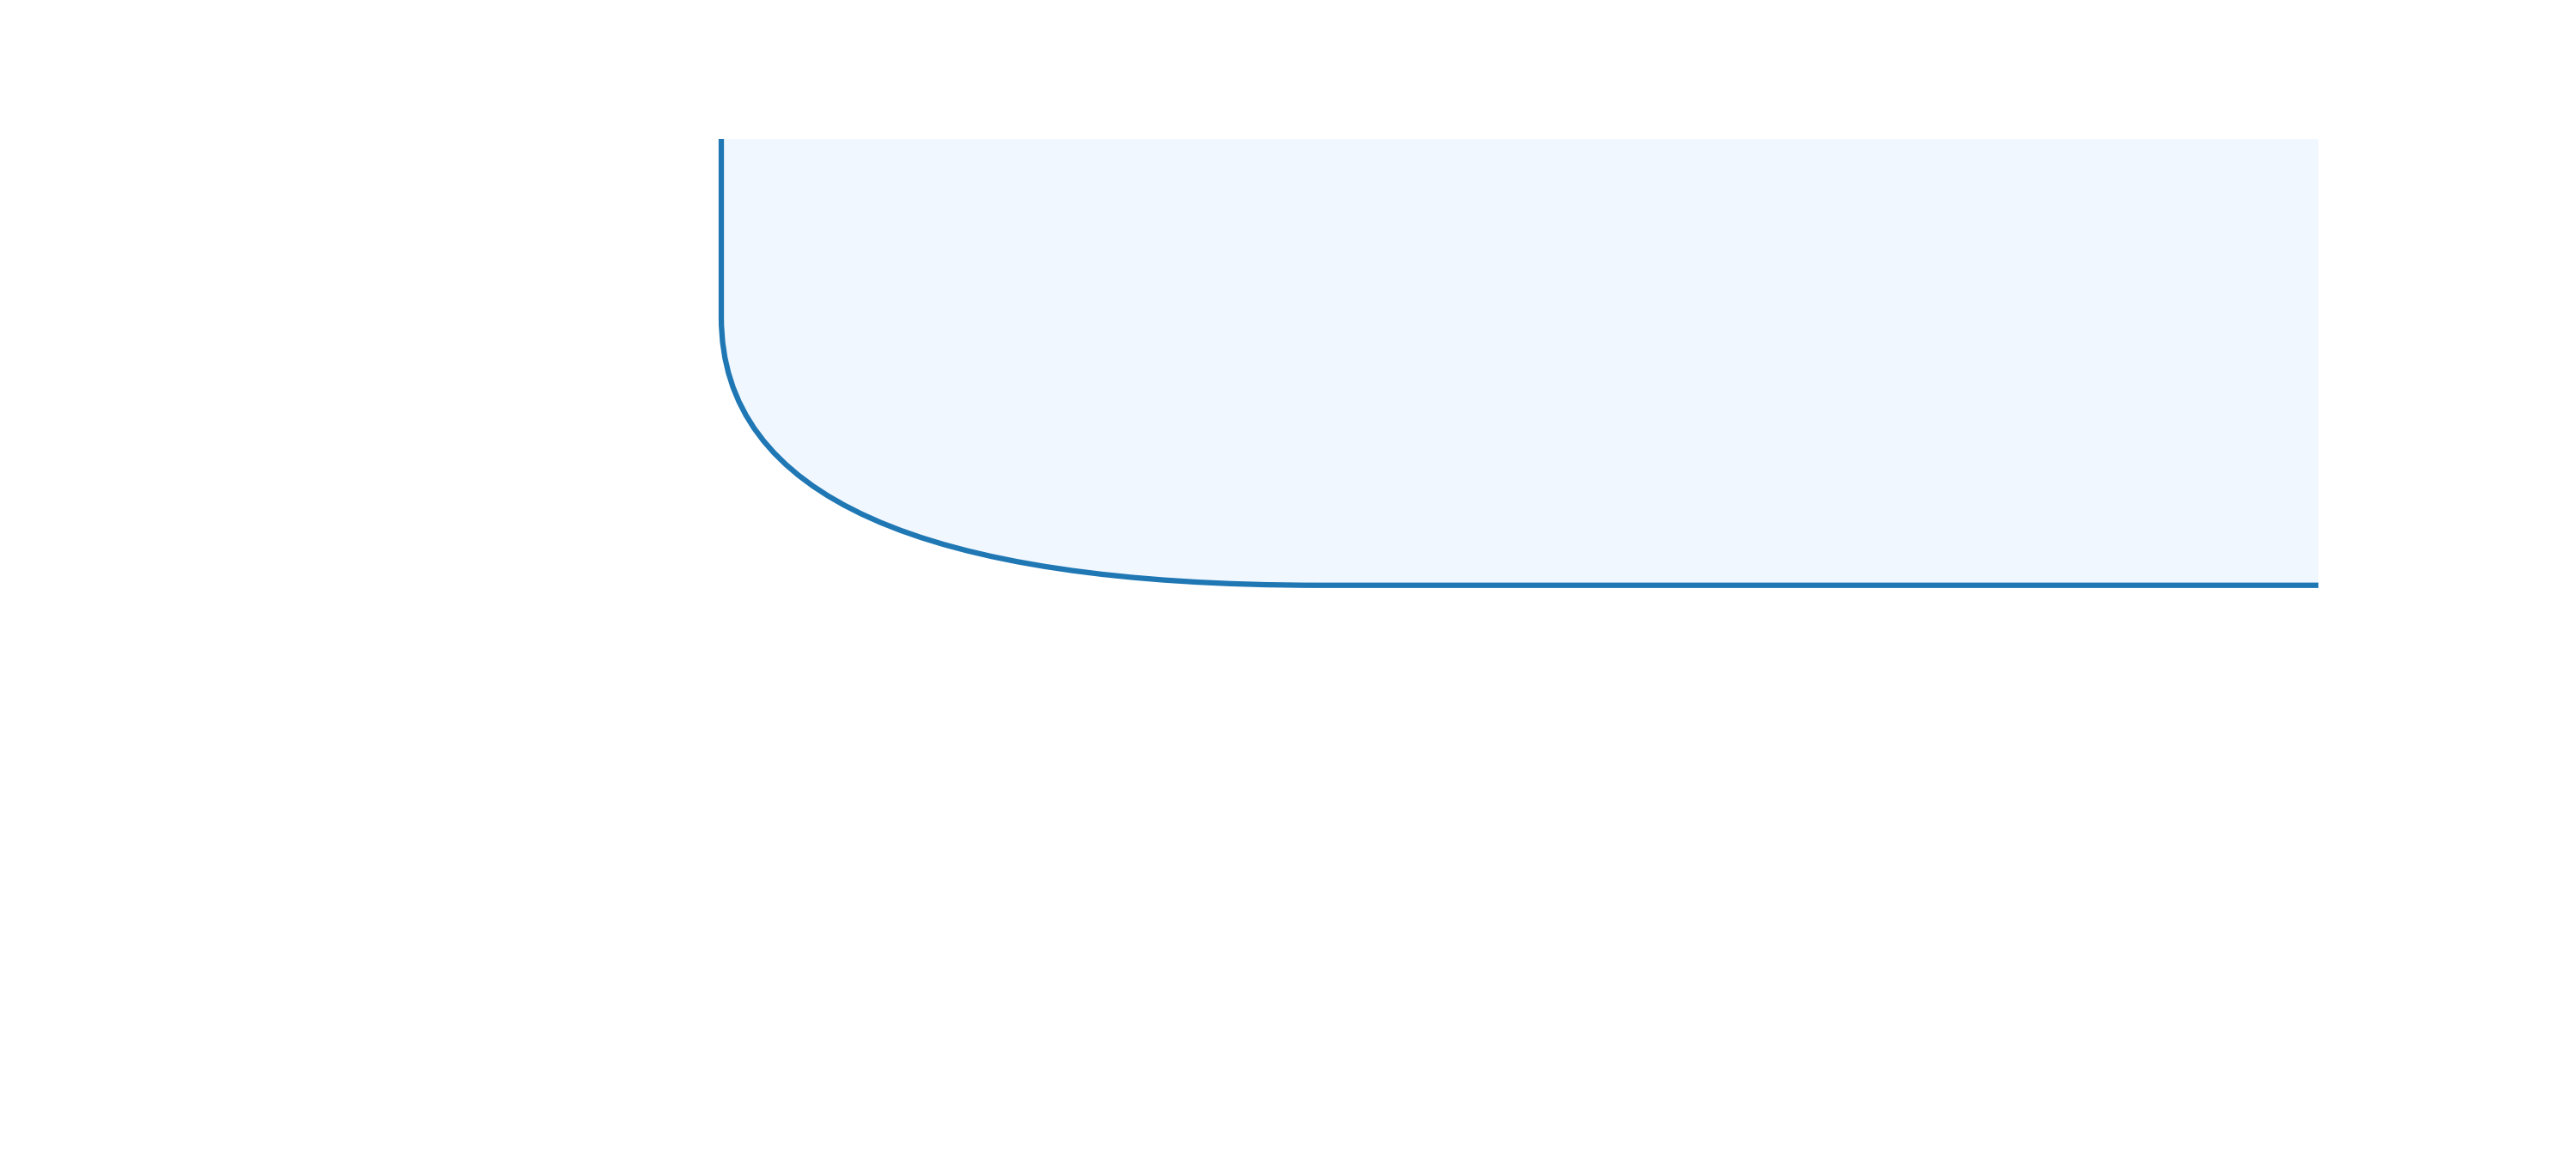
\includegraphics[width=0.9\textwidth]{gnn_application_landscape.png}
  \caption{GNN 在社交网络、分子化学、推荐系统中的应用概览。}
  \label{fig:gnn_application_landscape_cn}
\end{figure}
\FloatBarrier

\section*{延伸阅读}
\begin{itemize}
  \item Thomas N. Kipf \& Max Welling:《Semi-Supervised Classification with Graph Convolutional Networks》,ICLR 2017。
  \item Petar Veličković 等:《Graph Attention Networks》,ICLR 2018。
  \item Will Hamilton 等:《Inductive Representation Learning on Large Graphs》,NIPS 2017。
  \item Keyulu Xu 等:《How Powerful are Graph Neural Networks?》,ICLR 2019。
  \item He 等:《LightGCN: Simplifying and Powering Graph Convolution Network for Recommendation》,SIGIR 2020。
\end{itemize}

\end{document}
